\documentclass[xcolor={dvipsnames,usenames}]{beamer}
%\documentclass[xcolor={dvipsnames,usenames},handout]{beamer} % use this to compile w/o pauses
\mode<presentation>
{
\usetheme{Madrid}
\usecolortheme{default}
\setbeamertemplate{itemize items}[default]
\setbeamertemplate{enumerate items}[default]
\setbeamercovered{transparent}
\usefonttheme[onlymath]{serif}
}


\usepackage{microtype}
\usepackage[normalem]{ulem}
%\usepackage{hyperref}
%\hypersetup{colorlinks=true, urlcolor=Blue, citecolor=Green, linkcolor=BrickRed, breaklinks, unicode}

\usepackage[nocompress]{cite}
\usepackage{amsmath,mathtools}
\usepackage{euscript}
\usepackage{latexsym}
\usepackage{amssymb,stmaryrd}
\usepackage{enumerate}
\usepackage{algorithm,algorithmicx}
\usepackage[noend]{algpseudocode}
\renewcommand{\algorithmicrequire}{\textbf{Requirement:}}

\usepackage{graphicx}
\usepackage{epstopdf}
\usepackage{subcaption}
\graphicspath{{./fig/}}


\title{Efficient Algorithms for Geometric Partial Matching}
\author[Allen Xiao]
{
	Pankaj~K.~Agarwal \and
	Hsien-Chih~Chang \and
	Allen~Xiao
}
\institute[SoCG 2019]
{
	Department of Computer Science, Duke University
}
\date{June 2019}

% tweak wd=X\paperwidth to modify the footer dimensions in the madrid theme
\makeatletter
\setbeamertemplate{footline}{
  \leavevmode%
  \hbox{%
  \begin{beamercolorbox}[wd=.25\paperwidth,ht=2.25ex,dp=1ex,center]{author in head/foot}%
    \usebeamerfont{author in head/foot}\insertshortauthor\expandafter\ifblank\expandafter{\beamer@shortinstitute}{}{~~(\insertshortinstitute)}
  \end{beamercolorbox}%
  \begin{beamercolorbox}[wd=.55\paperwidth,ht=2.25ex,dp=1ex,center]{title in head/foot}%
    \usebeamerfont{title in head/foot}\insertshorttitle
  \end{beamercolorbox}%
  \begin{beamercolorbox}[wd=.2\paperwidth,ht=2.25ex,dp=1ex,right]{date in head/foot}%
    \usebeamerfont{date in head/foot}\insertshortdate{}\hspace*{2em}
    \insertframenumber/\inserttotalframenumber \hspace*{2ex}
  \end{beamercolorbox}}%
  \vskip0pt%
}
\makeatother


% make tables less packed
\renewcommand{\arraystretch}{1.5}
% get rid of caption labels
%\setbeamertemplate{caption}{\raggedright\insertcaption\par}
%\captionsetup[subfigure]{labelformat=empty}
% set beamer highlight color (alert)
\setbeamercolor{alerted text}{fg=BrickRed}

\newcommand{\mycite}[1]{{\color{LimeGreen}\lbrack #1\rbrack}}
\newcommand{\etal}{\textit{et~al.}}
\newcommand{\softO}{\widetilde{O}}
\newcommand{\reals}{\mathbb{R}}
\newcommand{\ints}{\mathbb{N}}
\newcommand\nats{\mathbb{N}}
\newcommand{\eps}{\varepsilon}
\DeclareMathOperator{\polylog}{polylog}
\DeclareMathOperator{\poly}{poly}
\newcommand{\flr}[1]{{\lfloor #1\rfloor}}
\DeclareMathOperator*{\argmax}{arg\,max}
\DeclareMathOperator*{\argmin}{arg\,min}
\DeclareMathOperator{\Vor}{Vor}
\DeclareMathOperator{\VorRegion}{VorRegion}

\def\abs#1{\mathopen| #1 \mathclose|}		% use instead of $|x|$
\def\norm#1{\mathopen\| #1 \mathclose\|}	% use instead of $\|x\|$

\DeclareMathOperator{\cost}{cost}
\newcommand{\tsupply}{\lambda}
\newcommand{\fsupply}{\phi}

\newcommand{\A}{{\color{red}A}}
\newcommand{\B}{{\color{blue}B}}
\newcommand{\M}{\EuScript{M}}
\newcommand{\tildeM}{\widetilde{\EuScript{M}}}
\newcommand{\X}{\EuScript{X}}

\def\EMPH#1{\textcolor{BrickRed}{{\emph{#1}}}}



\begin{document}


\begin{frame}
\maketitle
\end{frame}

% INTRO

% 01: gentle example, emphasize cost fn
\begin{frame}{Geometric (bipartite) matching}
% two point sets in 2d, show cost fn (distance exponentitated to constant)
\begin{figure}
\begin{center}
\includegraphics<1>[width=0.8\textwidth,page=1]{example}%
\includegraphics<2>[width=0.8\textwidth,page=2]{example}%
\includegraphics<3->[width=0.8\textwidth,page=3]{example}%
\end{center}
\end{figure}

\end{frame}

\begin{frame}{Geometric (bipartite) partial matching}
% only k pairs
\begin{figure}
\begin{center}
\includegraphics<1->[width=0.8\textwidth,page=4]{example}%
\end{center}
\end{figure}
\end{frame}

% 02: unit-cap MCF form
\begin{frame}{Geometric partial matching as unit-capacity min-cost flow}
% unit-capacity construction, note number of edges
\begin{figure}
\begin{center}
\includegraphics<1>[width=\textwidth,page=1]{pm-to-mcf}%
\includegraphics<2>[width=\textwidth,page=2]{pm-to-mcf}%
\includegraphics<3>[width=\textwidth,page=3]{pm-to-mcf}%
\includegraphics<4>[width=\textwidth,page=4]{pm-to-mcf}%
\includegraphics<5>[width=\textwidth,page=5]{pm-to-mcf}%
\includegraphics<6>[width=\textwidth,page=6]{pm-to-mcf}%
\includegraphics<7>[width=\textwidth,page=7]{pm-to-mcf}%
\includegraphics<8->[width=\textwidth,page=8]{pm-to-mcf}%
\end{center}
\end{figure}
\end{frame}

% 03*: select prior work
\begin{frame}{Issues for geometric perfect matching algorithms}
% many other geometric matching algs need triangle ineq and fail for q > 1, e.g. certain embedding into sparse graph
% for some others, unclear how to generalize to partial (e.g. divide and conquer AV04)
% notable: SA12 (only first power)
\begin{equation*}
|A| = r, \quad |B| = n, \quad A, B \subset \reals^2, \quad q \geq 1
\end{equation*}
\begin{equation*}
\min_{k \text{-matching } M}\sum_{(a, b) \in M} \|a - b\|^q
\end{equation*}
\vspace{-10pt}
\begin{figure}
\begin{center}
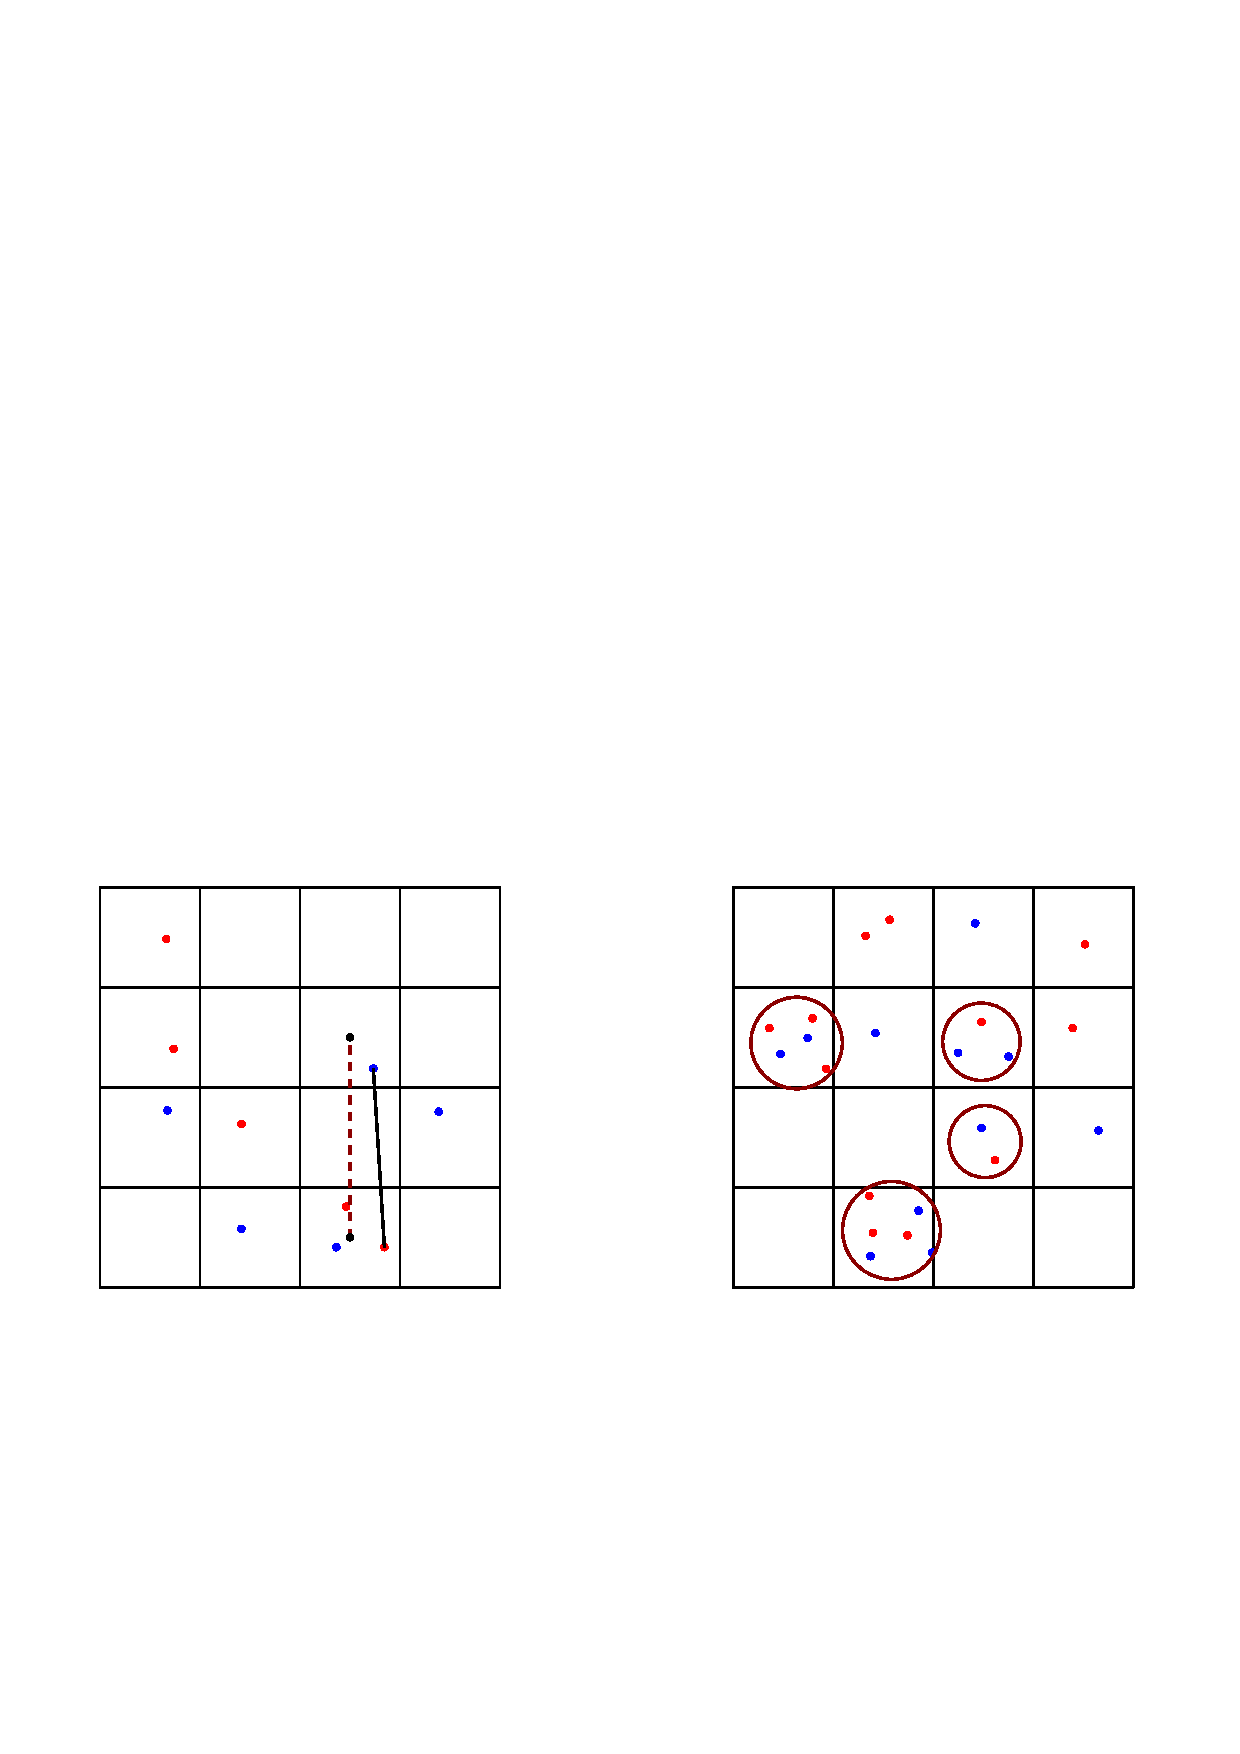
\includegraphics[width=0.9\textwidth,page=1]{perf_geom_issues}%
\end{center}
\end{figure}
\vspace{-5pt}
{\small For $q = 1$, [Sharathkumar-Agarwal]: $(1+\eps)$-approx. in $O(n\poly(1/\eps, \log n))$ time.}
\end{frame}

% 04: new results for partial, geom. based on prior work. present 1,2 only
\begin{frame}{Partial matching algorithms (non-geometric)}
% non-geom: Hungarian, RT/GHKT cost scaling,
% geometrized:
% Hungarian+BCP (Vaidya, KMRSS)
% cost-scaling+BCP
\begin{equation*}
|A| = r, \quad |B| = n, \quad A, B \subset \reals^2, \quad q \geq 1 
\end{equation*}
\begin{equation*}
\min_{k \text{-matching } M}\sum_{(a, b) \in M} \|a - b\|^q
\end{equation*}
\begin{itemize}
\item Hungarian algorithm [Kuhn]: $O(kn^2 + k^2\log r)$
\item Cost-scaling [Ramshaw-Tarjan, Goldberg~\etal]: $O(n^2\sqrt{k}\log(kC))$ (integer costs),
	or $O(n^2\sqrt{k})$ time per cost scale. \pause
	\begin{itemize}
	\item After reduction, $\log(n^q/\eps)$ cost scales for a $(1+\eps)$-approx. \pause
	\end{itemize}
\end{itemize}
\vspace{10pt}
Using dynamic bichromatic closest pair (BCP) data structures:
\begin{itemize}
\item Hungarian algorithm: $O(kn\polylog(n))$
\item Cost-scaling: $O(n\sqrt{k}\polylog(n))$ time per cost scale.
\end{itemize}
\end{frame}

% our results 1
\begin{frame}{Our results}
% Hungarian+BCP
% cost-scaling+BCP
Previous:
\begin{itemize}
\item Hungarian algorithm w/ BCP: $O(kn\polylog(n))$
\item Cost-scaling w/ BCP: $O(n\sqrt{k}\polylog(n))$ time per cost scale.
\end{itemize}
\pause
\vspace{10pt}

New:
\begin{enumerate}
\item Hungarian algorithm: $O((n+k^2)\polylog(n))$ time, exact.
\item Cost-scaling: $O((n+k\sqrt{k})\polylog(n))$ time per cost scale, $(1+\eps)$-approx.
\pause
\vspace{10pt}
\item Geometric Transportation: $O(\min(n^2, nr^{3/2})\polylog(n))$ time, exact.
\end{enumerate}
\end{frame}

% HUNG

% 05: Hungarian algorithm and least-cost augmentation
% TODO talk about potentials?
\begin{frame}{Hungarian algorithm}
\end{frame}

% 06: Hungarian search with BCP
\begin{frame}{Hungarian search, with BCP}
\end{frame}

% 08*: problem: initializing the BCP data structure (why not persistence?)
\begin{frame}{Problem: BCP initialization}
\end{frame}

% 09*: rewinding --> k^2polylogn time per augmentation, one-time npolylogn pre
\begin{frame}{Rewinding}
\end{frame}

% 10: potential changes + Vaidya?
\begin{frame}{Potential updates}
\end{frame}

% COST-SCALE

% our results 2
\begin{frame}{Our results}
% Hungarian+BCP
% cost-scaling+BCP
\end{frame}

% 11: cost-scaling unit-cap MCF
\begin{frame}{Partial matching by cost-scaling}
\end{frame}

% 12: changing scales (2\eps to \eps, losing circulation)
\begin{frame}{Initial $\theta$-optimal pseudoflow of a scale}
\end{frame}

% 13: refinement by blocking flows (more of the same, \sqrt{k} per scale, O(k) size per blocking)
\begin{frame}{Refinement by blocking flows}
\end{frame}

% 14*: new problem: number of relaxations could be \Omega(n) (example); compare vs Hung
\begin{frame}{Hungarian search dead ends}
\begin{enumerate}
\item There can be $\Omega(n)$ relaxations even if $k$ is very small.
%TODO
\end{enumerate}
\end{frame}

% 15: dead/alive nodes, alive paths. "really want to query minimizing alive path instead", "don't track their potential"
\begin{frame}{Dead or alive}
\end{frame}

% 16: alive paths in the BCP
\begin{frame}{Hungarian search over alive paths}
\end{frame}

% 17: # relaxations = O(|supp(f)|) = O(k)
\begin{frame}{How many relaxations now?}
\end{frame}

% 18*: dead node potentials
\begin{frame}{Dead node potentials}
\end{frame}

% 19: punchline running time: per-scale npolylogn pre, k\sqrt{k}polylogn per, O(log(n^q/\eps)) scales
\begin{frame}{Cost-scaling time summary}
\end{frame}

%TODO

% end slide
\begin{frame}{The End}
\begin{center}
	Thank you.
\end{center}
\end{frame}



%SECTION: pmt

% gentle example + equation

%\begin{frame}{Example}
%\begin{figure}
%\begin{center}
%\includegraphics<1>[width=\textwidth,page=1]{pmt_example}%
%\includegraphics<2>[width=\textwidth,page=2]{pmt_example}%
%\includegraphics<3>[width=\textwidth,page=3]{pmt_example}%
%\includegraphics<4>[width=\textwidth,page=4]{pmt_example}%
%\includegraphics<5>[width=\textwidth,page=5]{pmt_example}%
%\includegraphics<6>[width=\textwidth,page=6]{pmt_example}%
%\includegraphics<7->[width=\textwidth,page=7]{pmt_example}%
%\end{center}
%\end{figure}
%\begin{itemize}
%\item<7-> Find the minimum-cost matching over all translations.
%\end{itemize}
%\end{frame}


%\begin{frame}[allowframebreaks]{Citations}
%\tiny
%\bibliography{ref}
%\bibliographystyle{alpha}
%\end{frame}

\end{document}
